\providecommand{\main}{../../../..}
\documentclass[\main/dresen_thesis.tex]{subfiles}

\begin{document}
  \begin{figure}[htbp]
    \centering
    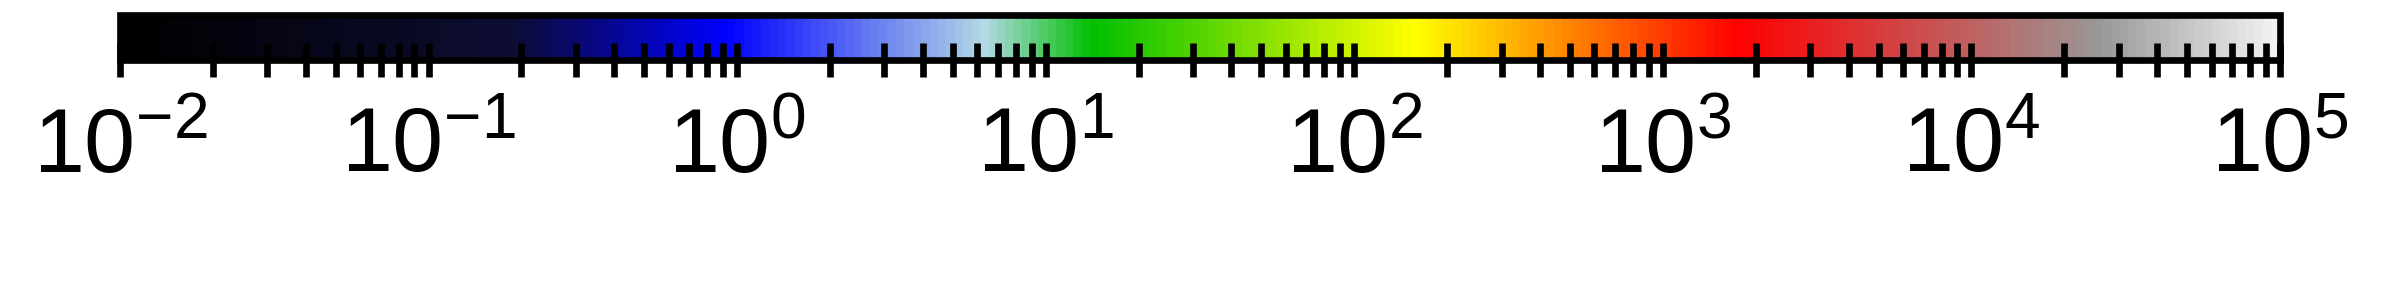
\includegraphics{monolayers_GISANSsimulation_SVcbar}
    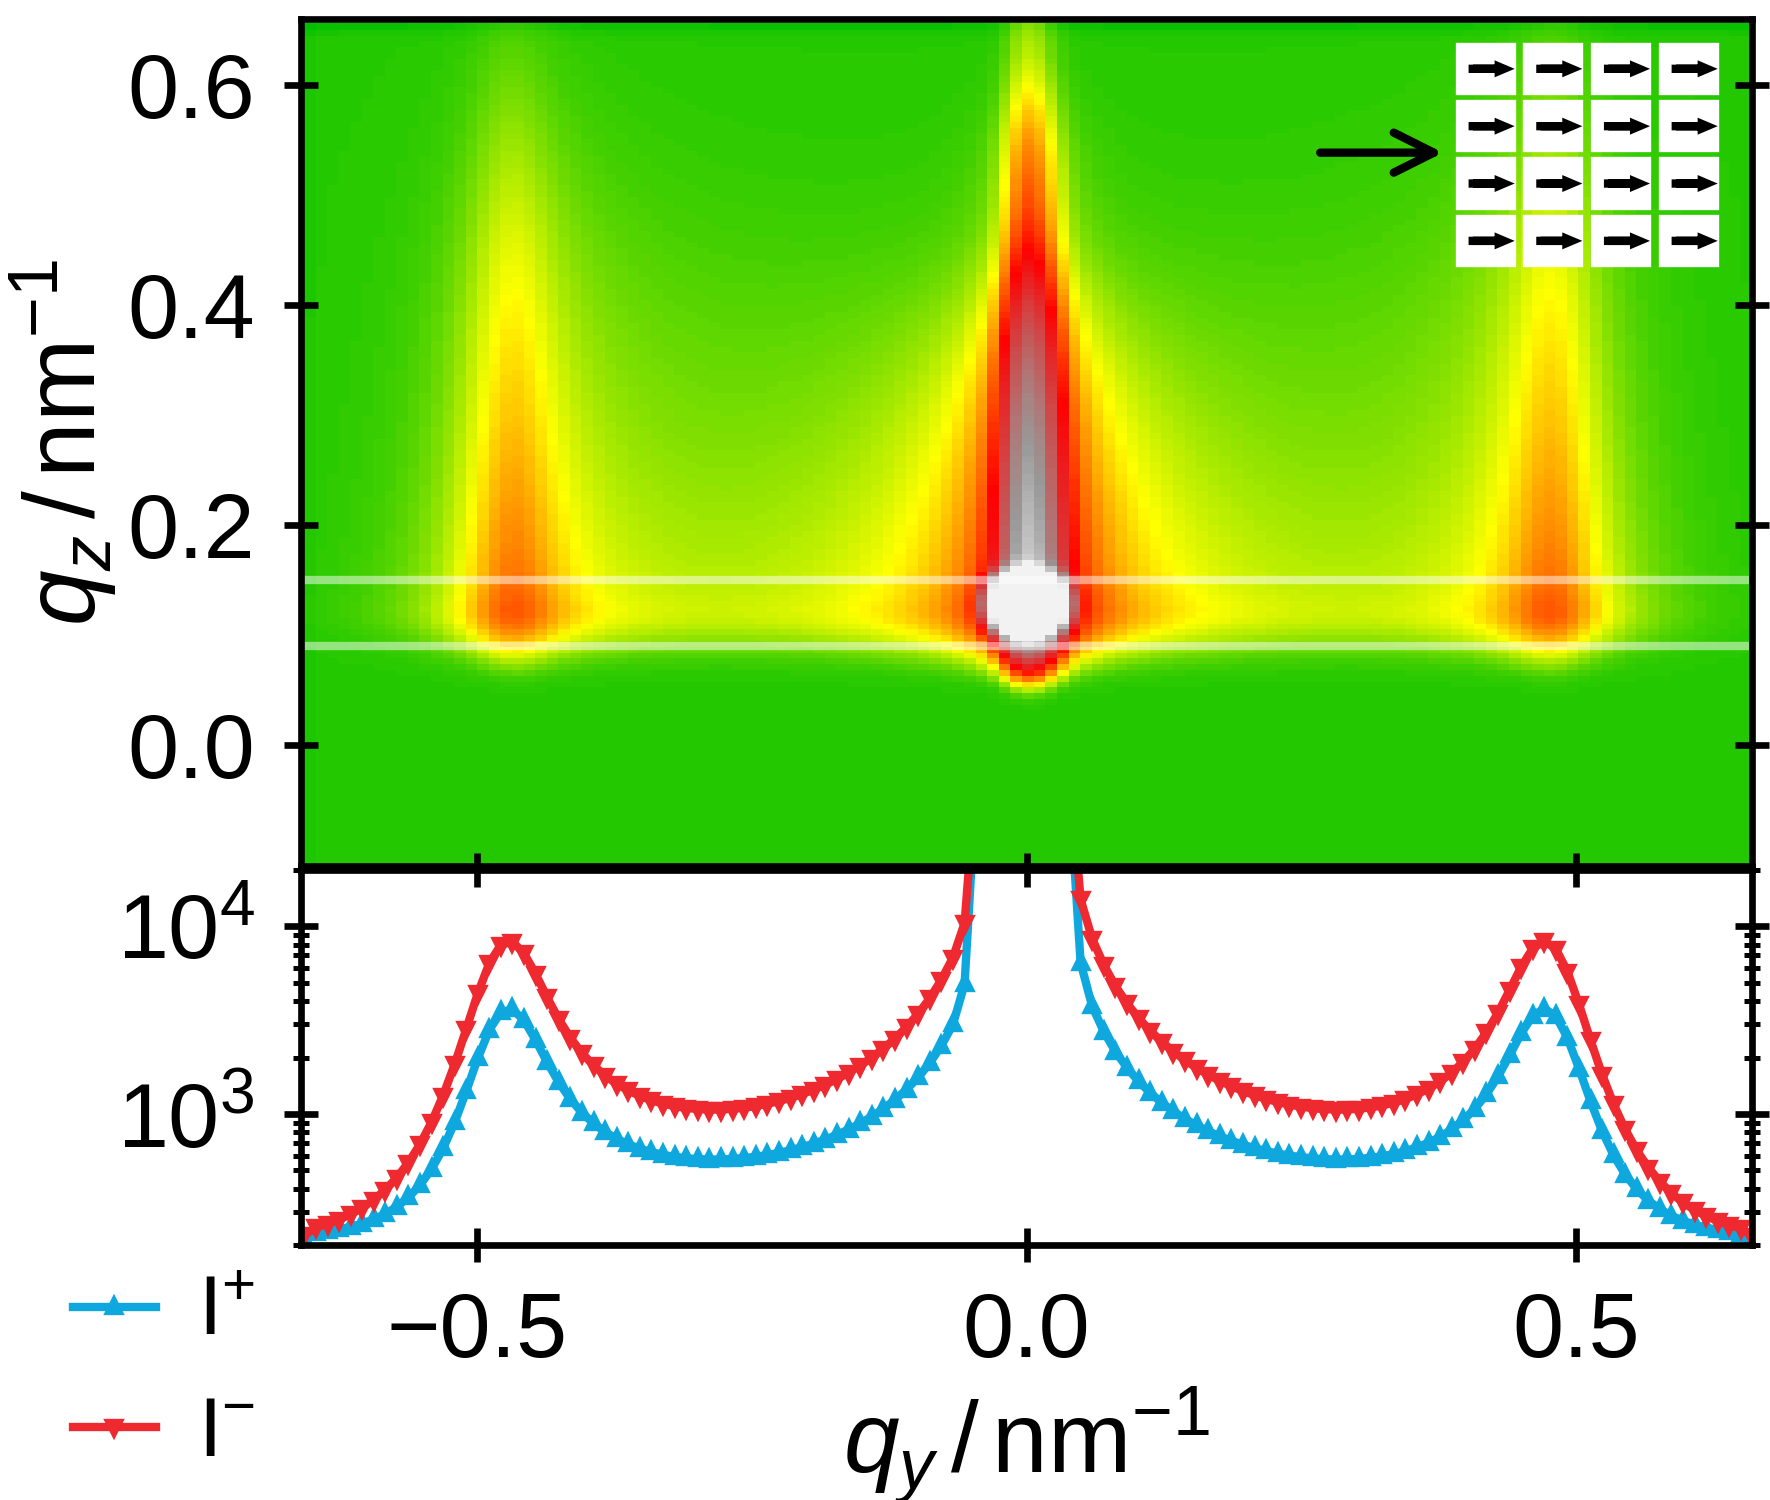
\includegraphics{monolayers_GISANS_ParacrystalSimulationMagParallelBeam}
    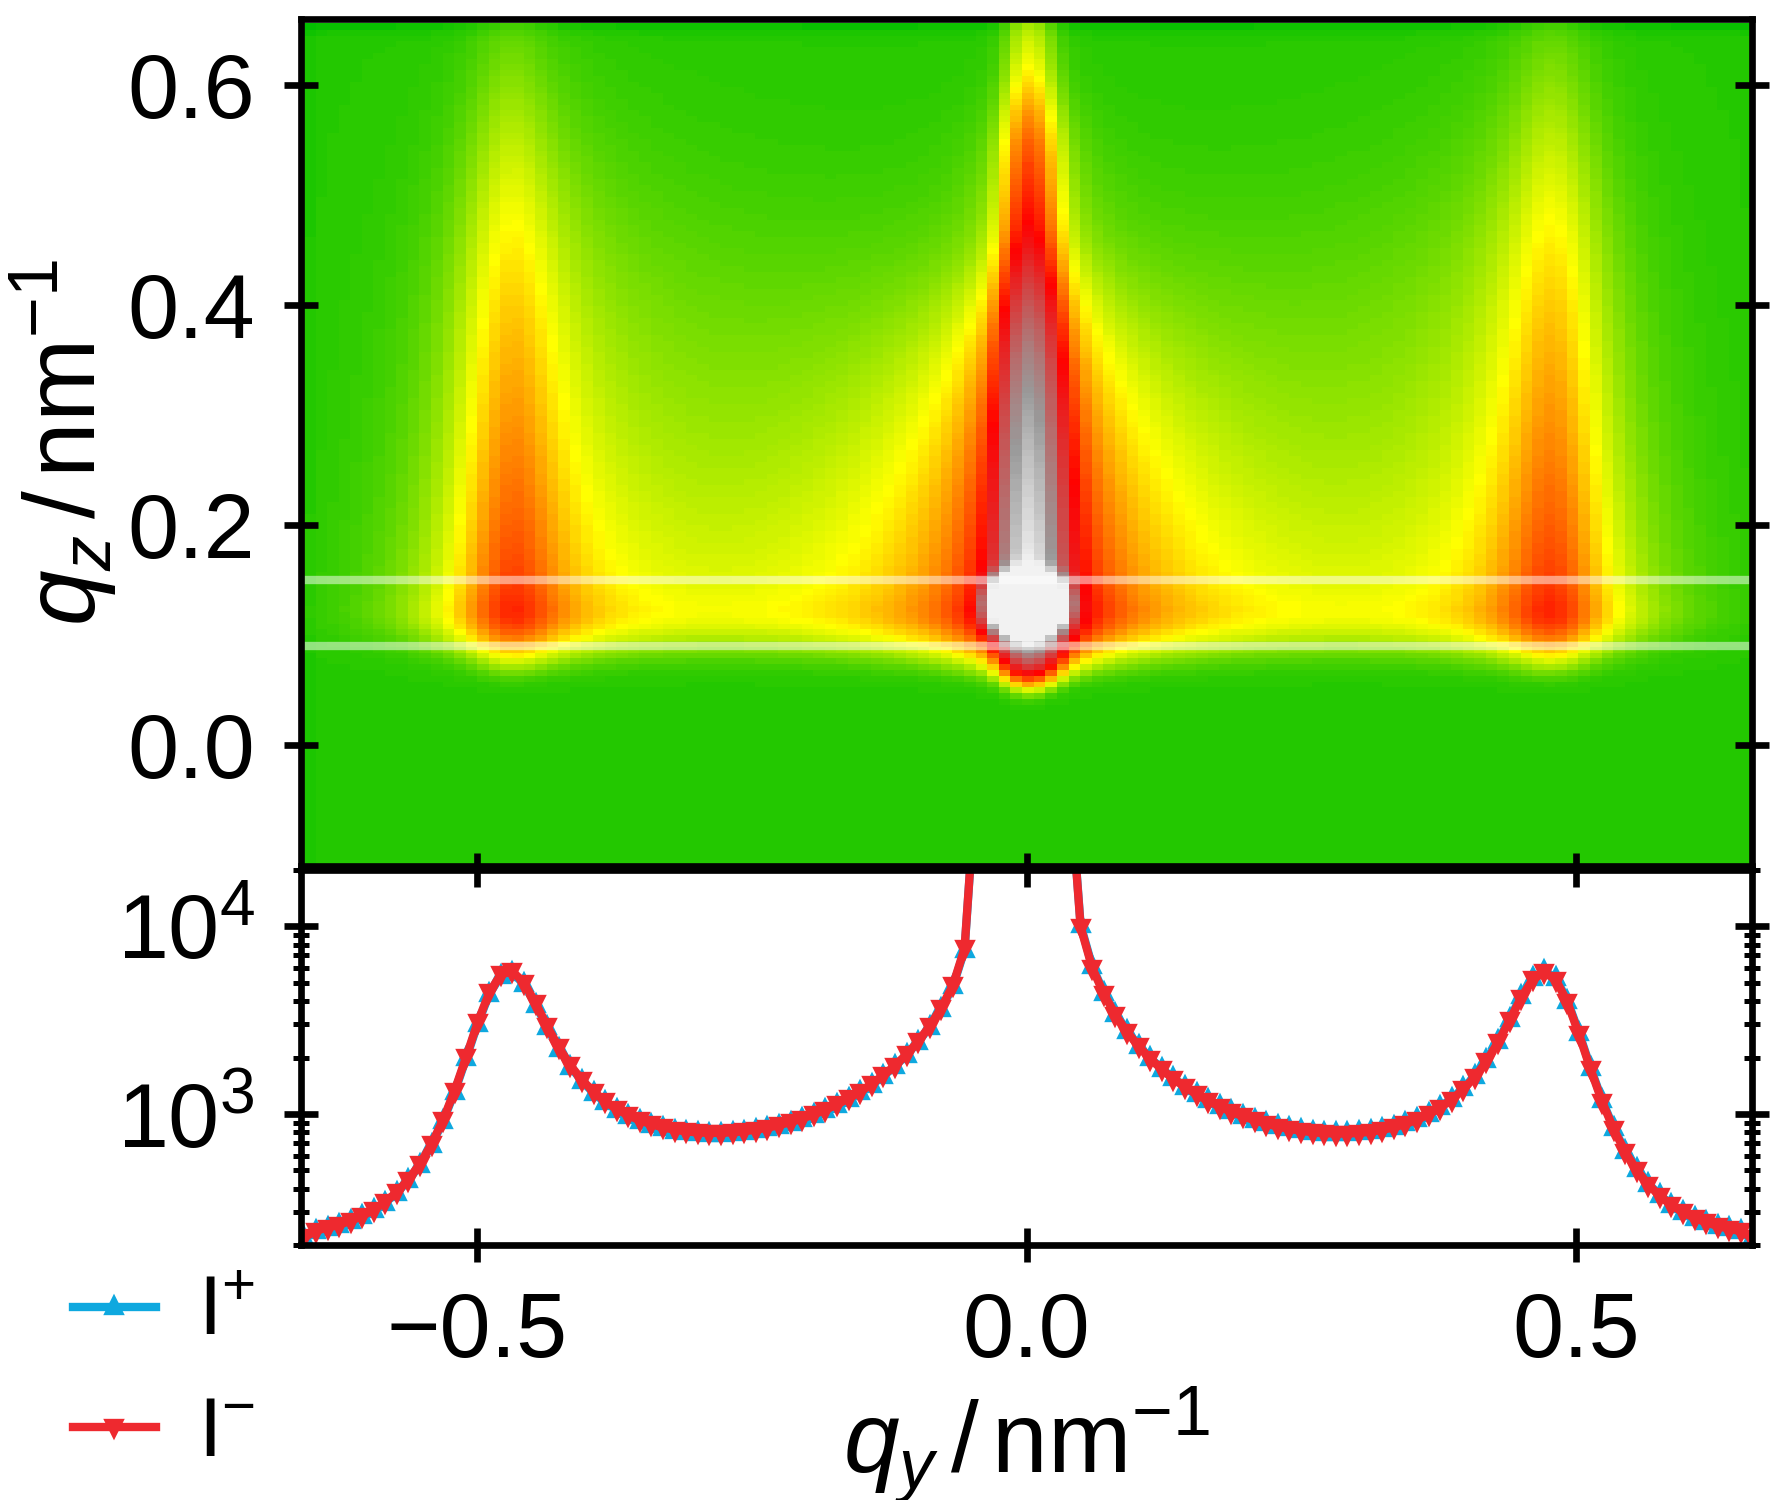
\includegraphics{monolayers_GISANS_ParacrystalSimulationMagPerpendicularBeam}
    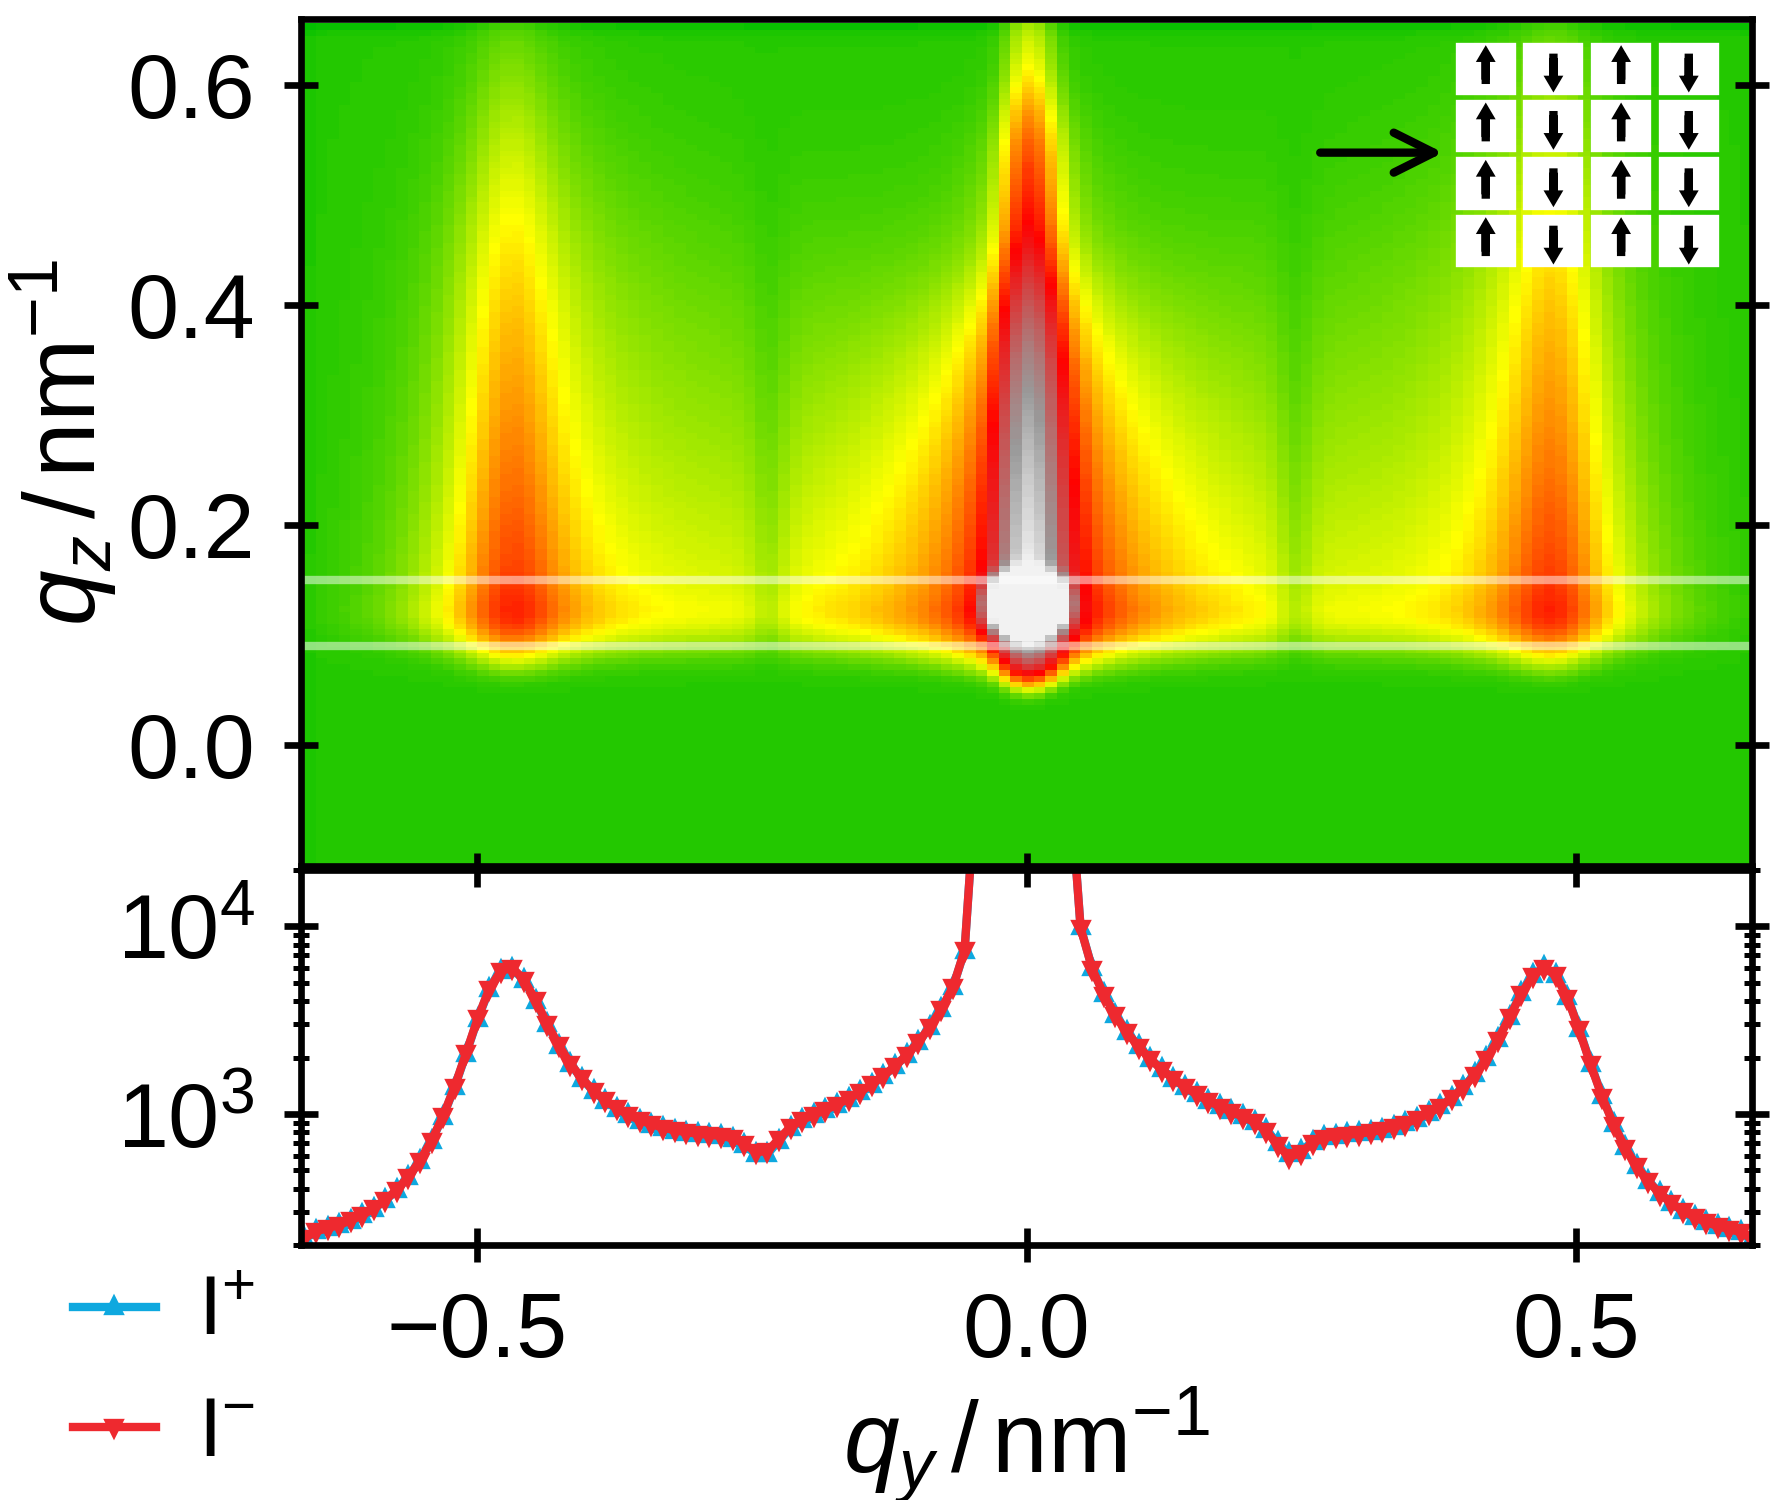
\includegraphics{monolayers_GISANS_ParacrystalSimulationMagAlternatingPerpendicularToBeam}
    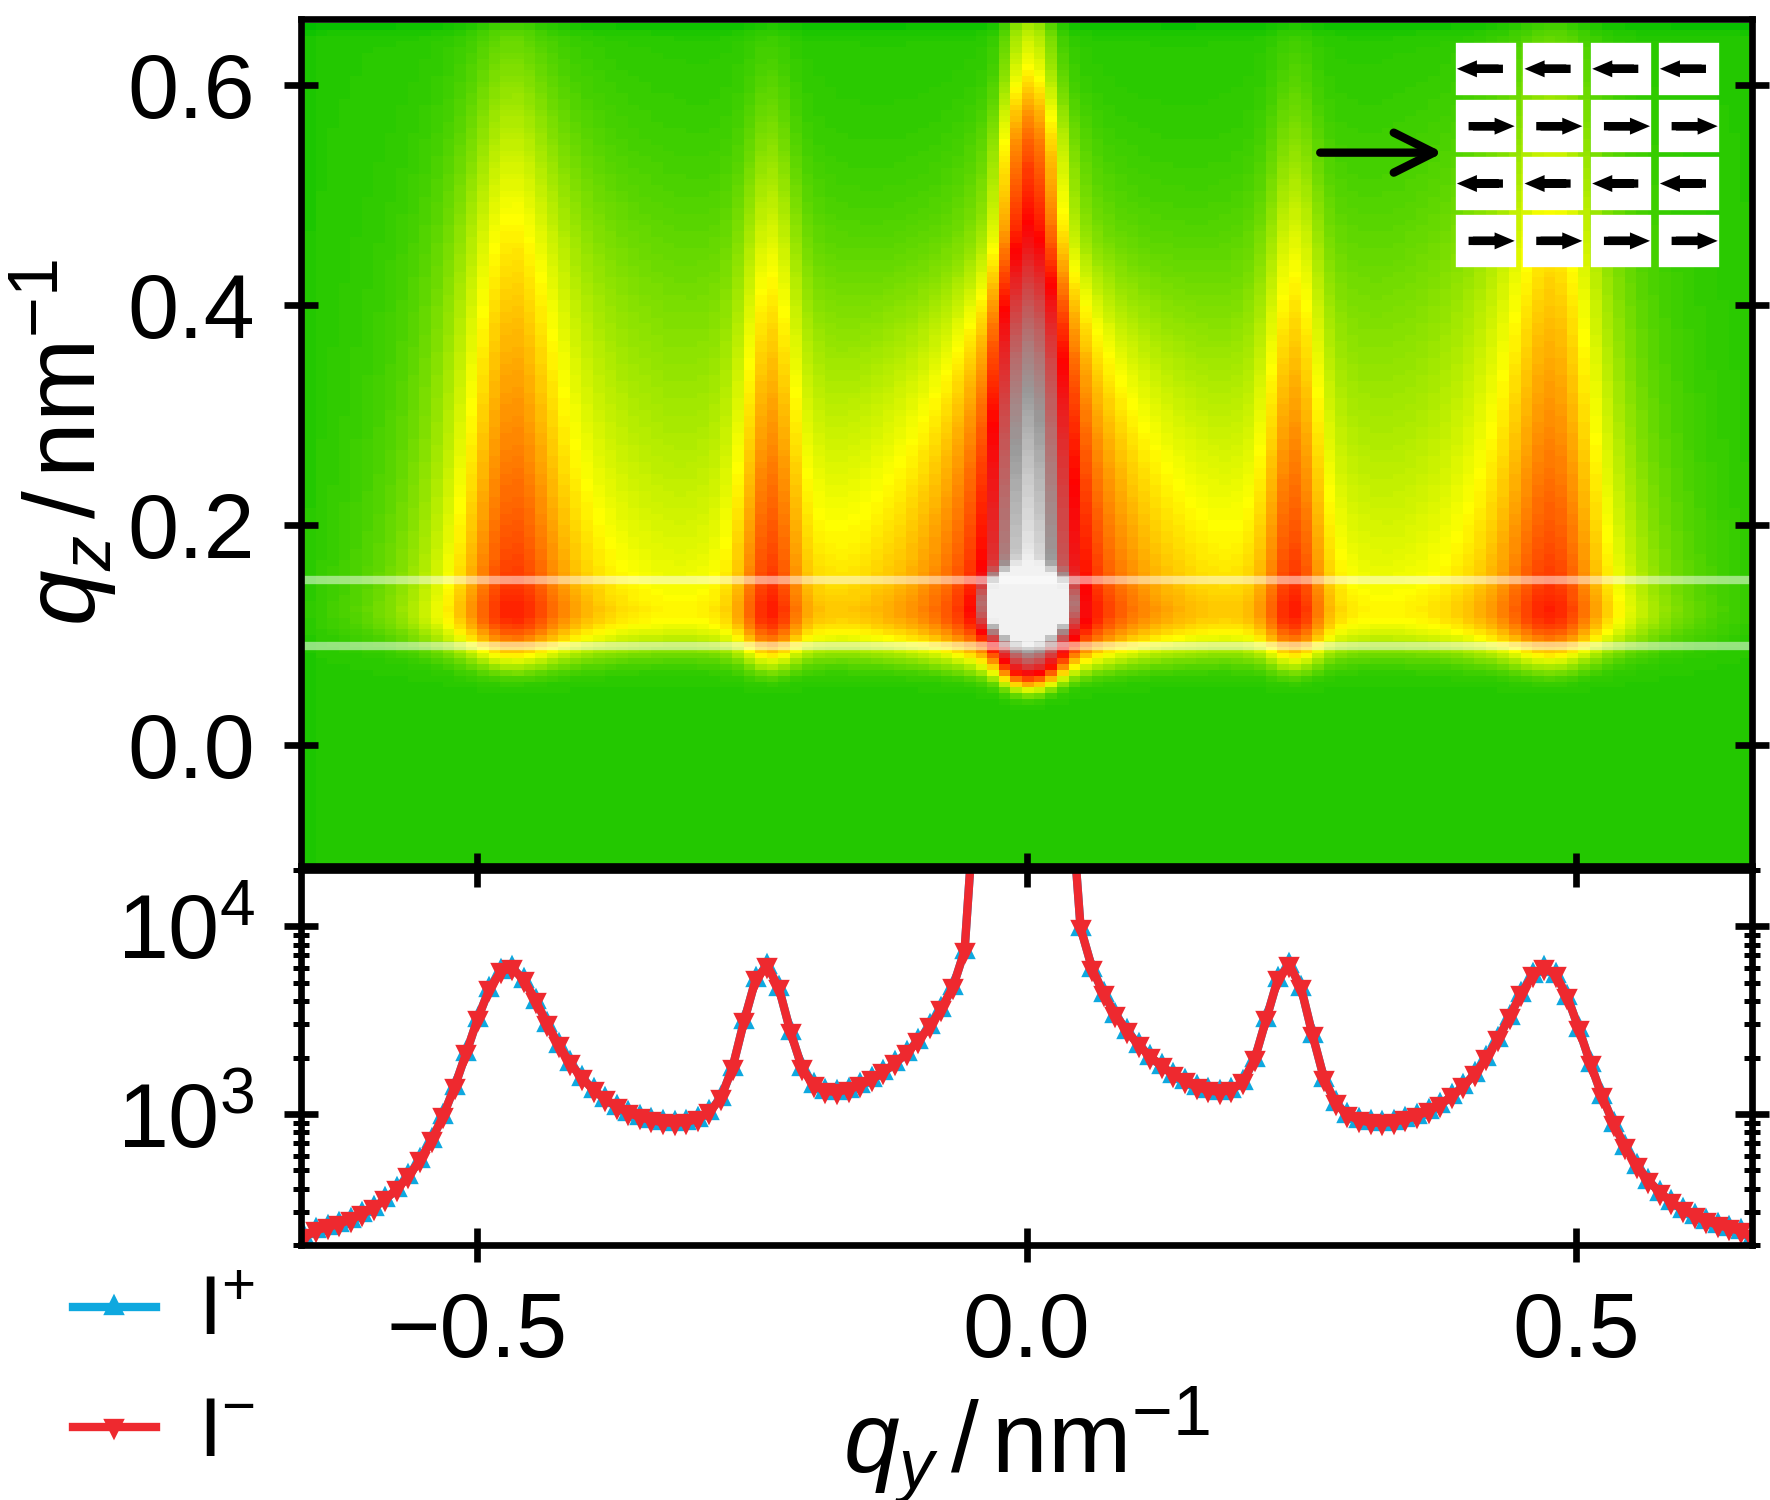
\includegraphics{monolayers_GISANS_ParacrystalSimulationMagAlternatingToBeam}
    \caption{\label{fig:monolayers:gisans:simulationAlternating}Simulation made with BornAgain \cite{Burle_2018_borna} of four limiting cases of magnetic configurations on a square lattice: homogeneously magnetized along the beam direction (upper left), homogeneously magnetized perpendicular to the beam direction (upper right), super antiferromagnetic coupling along the beam direction (lower left) and super antiferromagnetic coupling perpendicular to the beam (lower right). Shown are the detector images of $I^{+}$ and the projection from the Yoneda band for both $I^{+}$ and $I^{-}$. The beam polarization is set parallel to the beam direction for the simulation, which is marked by a large black arrow.}
  \end{figure}
  Polarized GISANS is used to discuss whether a macroscopic super antiferromagnetic state is present in the sample ML-Ac-CoFe-C-2, which consists of nanocubes ordered in a square array.
  As a technique to resolve lateral correlations in a nanostructure that is also sensitive to the magnetic structure, GISANS is ideal for this purpose as it is expected that a super antiferromagnetic structure shows additionally to the nuclear scattering peaks with the period of the lattice, magnetic scattering with the double period.
  Due to symmetry this effect should also be independent of the neutron polarization and therefore visible in both channels $I^{+}$ and $I^{-}$.

  The expected scattering from different magnetic configurations has been simulated using the BornAgain software, with the results shown in \reffig{fig:monolayers:gisans:simulationAlternating}.
  For the simulation, the structure described in \refsec{sec:monolayers:structure:squareArrayParacrystalGISAXS} is used, and a magnetization of $444 \unit{kA \, m^{-1}}$ is assumed for the nanocubes following the result from \refsec{sec:monolayers:nanoparticle:sas}.
  To have the magnetic configuration well-defined with the square array lattice structure, no orientation average of the square array with respect to the beam direction is performed for the simulation.

  Four cases of magnetic configurations in the square array plane are differentiated, two for super ferromagnetic states and two for super antiferromagnetic states.
  When the sample is homogeneously magnetized along the beam direction in the coherent scattering domain, a magnetic splitting is expected between the $I^{+}$ and $I^{-}$.
  If the sample is homogeneously magnetized perpendicular to the beam direction, no splitting should be observed.
  For the super antiferromagnetic configurations, one can also consider whether the antiferromagnetic coupling is along the beam direction or perpendicular to it.
  In the first case, no significant difference to the purely nuclear case would be observable up to a possible small dip at the $q_y$ value corresponding to the double period of the square array.
  In the second case however, a strong additional peak from the super-antiferromagnetic structure should emerge half way between the direct beam and first nuclear peak.
  The observation of such an additional peak would therefore be a direct evidence of the emergent SAFM state.
  \\

  \begin{figure}[tb]
    \centering
    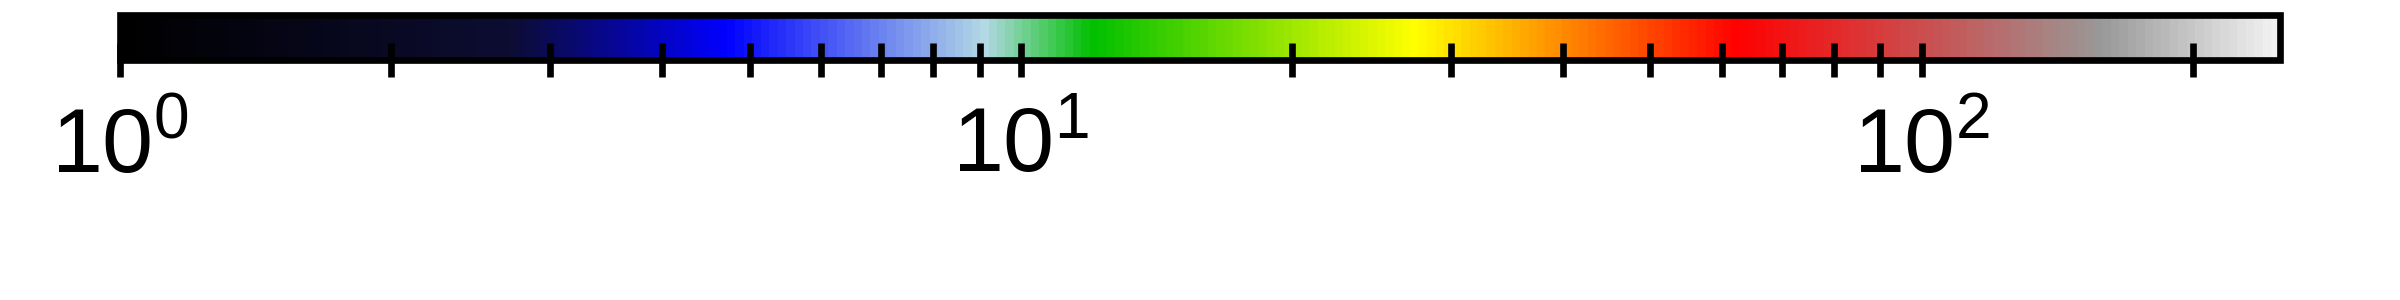
\includegraphics{monolayers_ML-Ac-CoFe-C_GISANS_SVcbar_parallelBeam}
    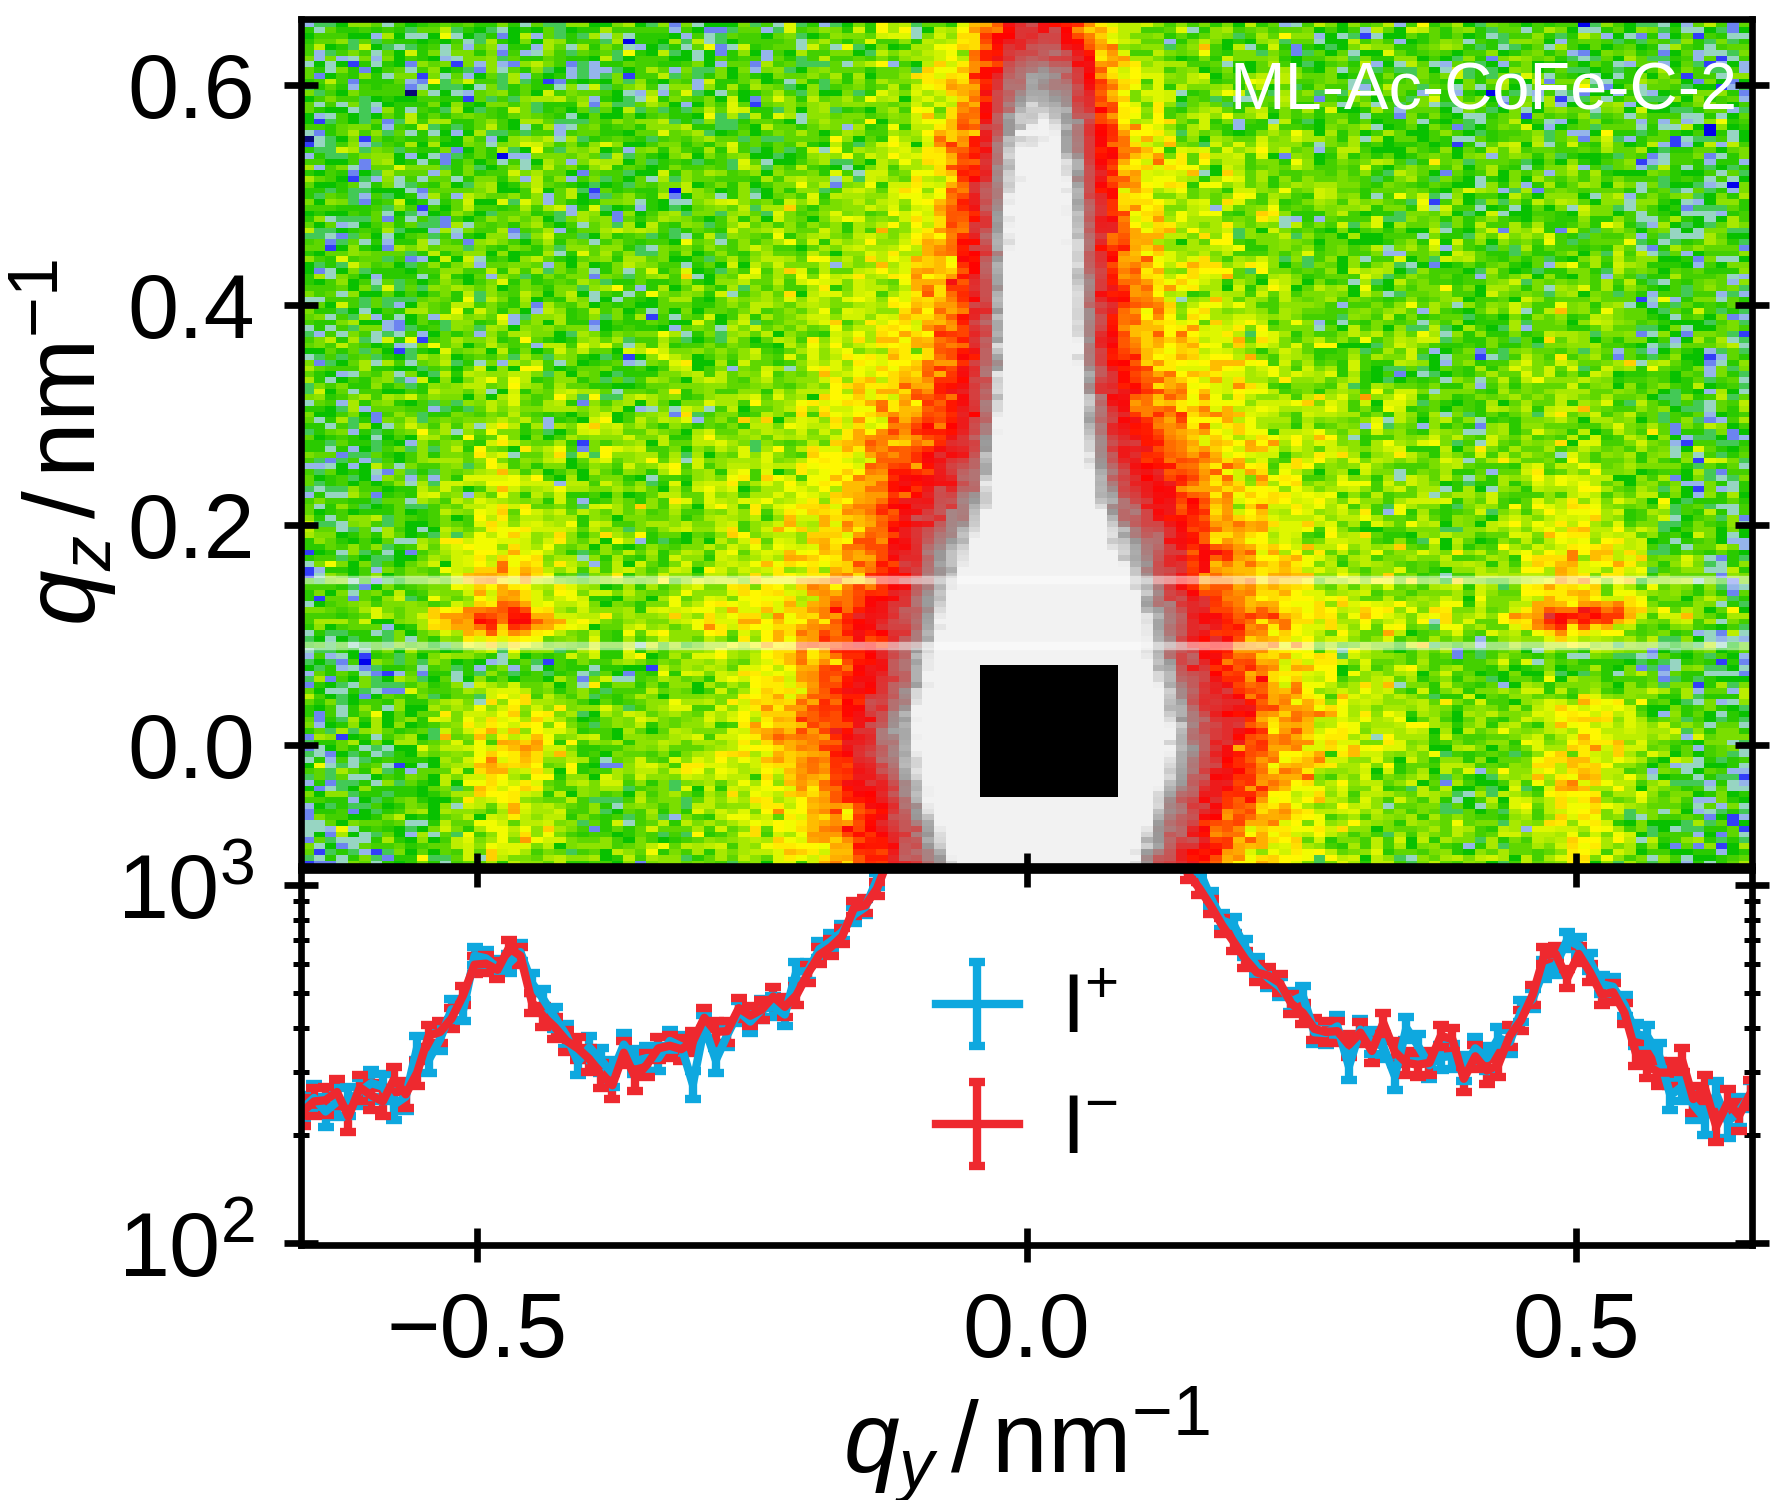
\includegraphics{monolayers_GISANS_ML-Ac-CoFe-C-2_ZFC5K_GF}
    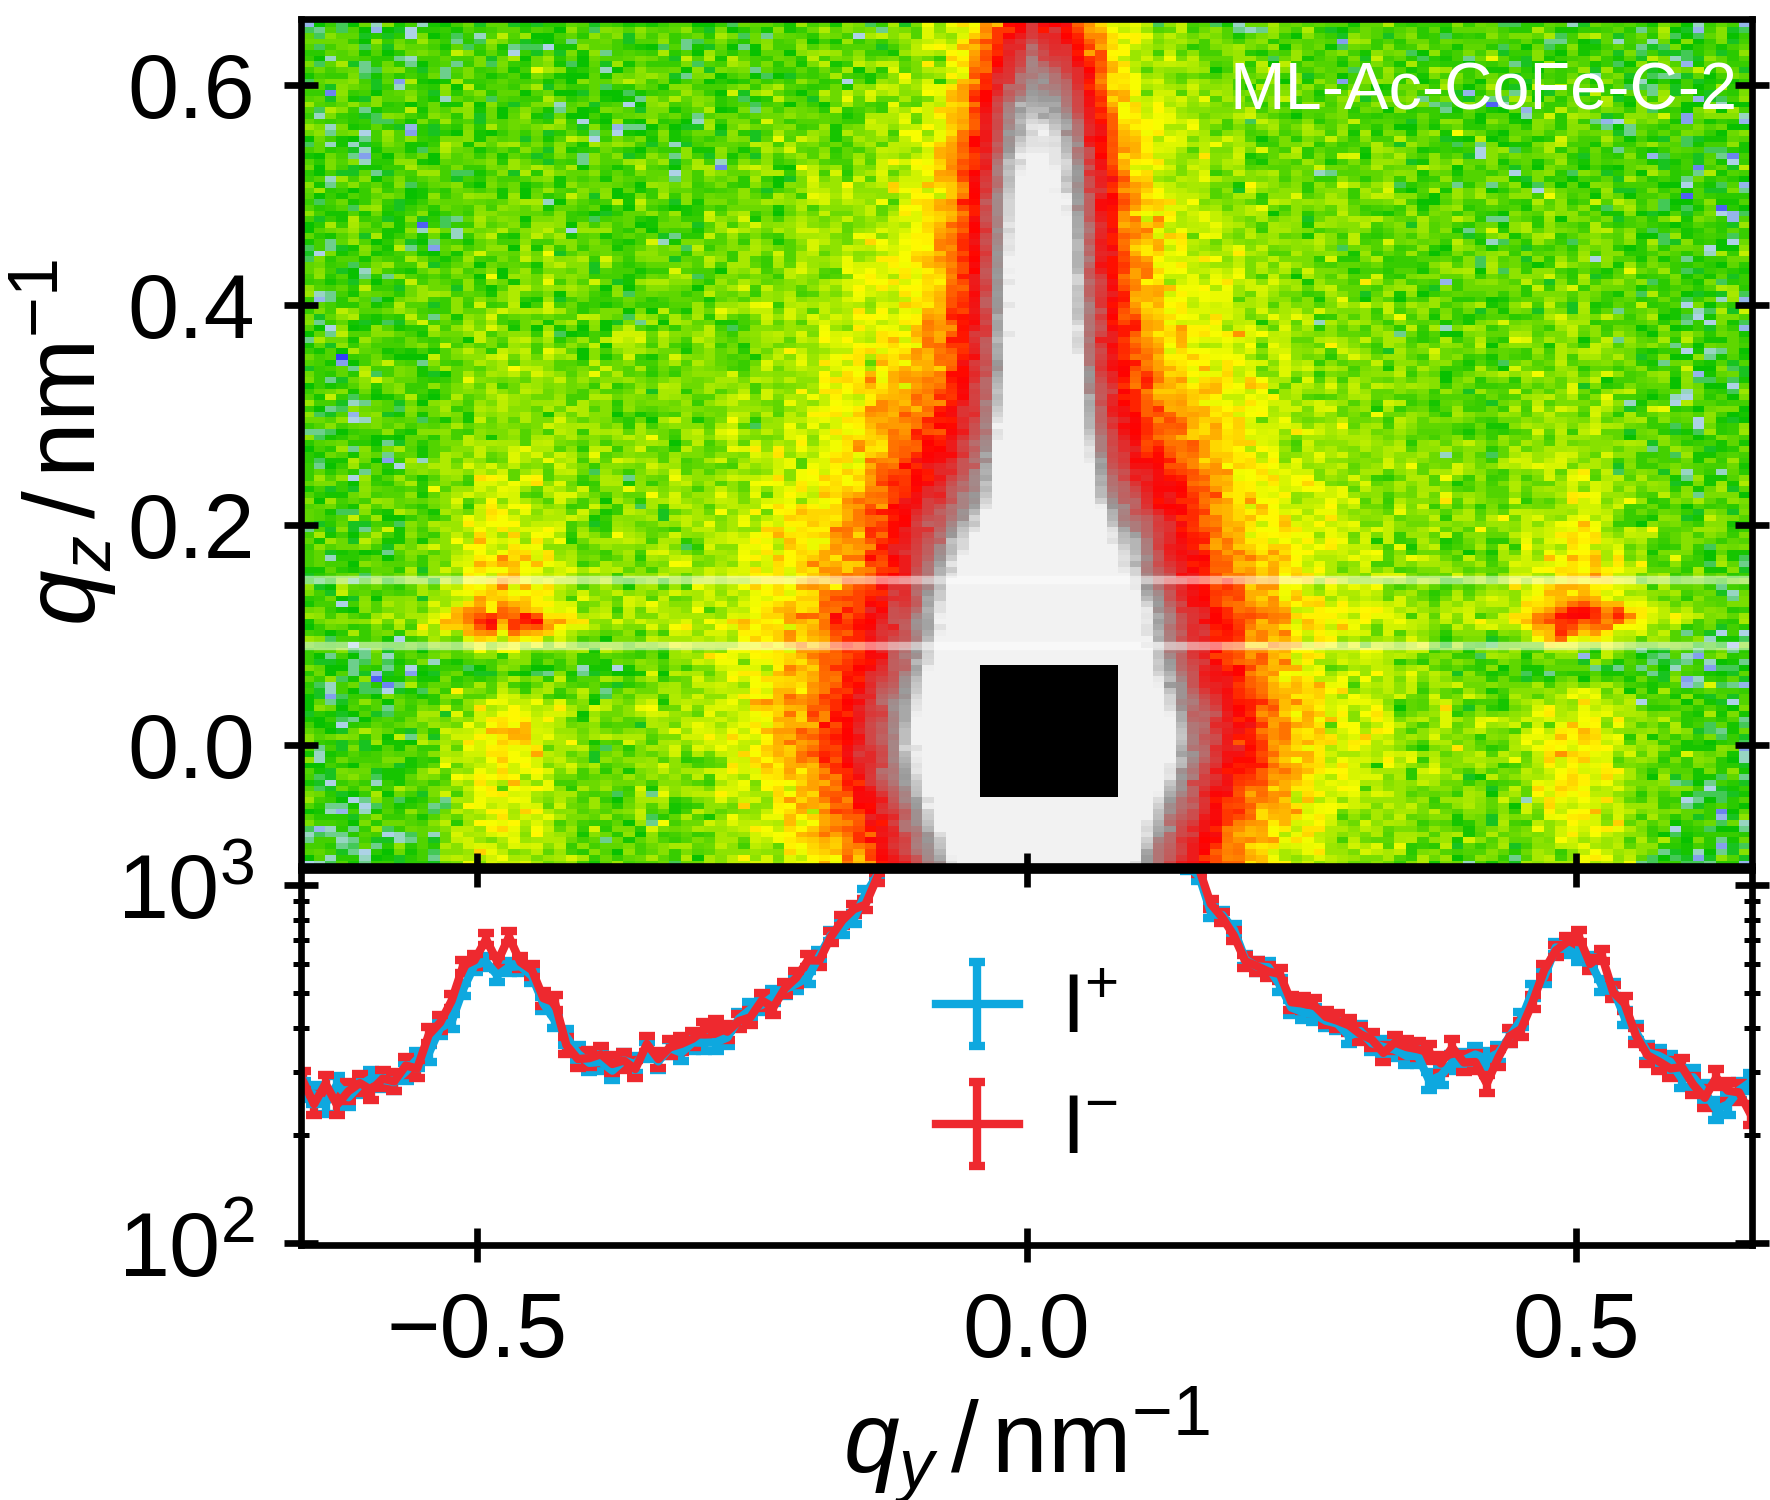
\includegraphics{monolayers_GISANS_ML-Ac-CoFe-C-2_ZFC5K_Remanence}
    \caption{\label{fig:monolayer:magneticStructure:polGisans5KZFC}Polarized grazing-incidence small-angle neutron scattering of ML-Ac-CoFe-C-2 after zero-field cooling to $5 \unit{K}$. Left is the detector image $I^{+}$ measured at guide field ($5 \unit{mT}$) after zero-field cooling and right the detector image of $I^{+}$ in remanence after exposing the sample to a field of $4 \unit{T}$ parallel to the neutron beam and subsequently turning back to guide field. The lower plots show the projection of the Yoneda band for both $I^{+}$ and $I^{-}$ and the nuclear peak position and half it's value are marked by black lines.}
  \end{figure}

  In \reffig{fig:monolayer:magneticStructure:polGisans5KZFC} the polarized GISANS images ($I^{+}$) are shown, which were measured at D33 for ML-Ac-CoFe-C-2 after zero-field cooling to $5 \unit{K}$ in the initial state and at remanence after the application of a $4 \unit{T}$ field parallel to the beam with a guide field of $5 \unit{mT}$ in both cases.

  In the Yoneda band, the first order nuclear peak is clearly visible in both cases around $0.5 \unit{nm^{-1}}$.
  Within the counting error, no significant difference is visible between the two polarization channels.
  From the nuclear peak position, the expected position for the super antiferromagnetic peak at the double period is marked, where however no significant peak is visible.
  This means that neither a super ferromagnetic nor a super antiferromagnetic state is clearly visible in this case.
  This is a bit surprising, as the magnetization measurement in \refsec{sec:monolayers:magneticStructure:vsm} suggests a strong magnetization at remanence, and therefore a significant number of nanoparticles should still be aligned with the direction of the applied magnetic field during saturation.

  \begin{figure}[tb]
    \centering
    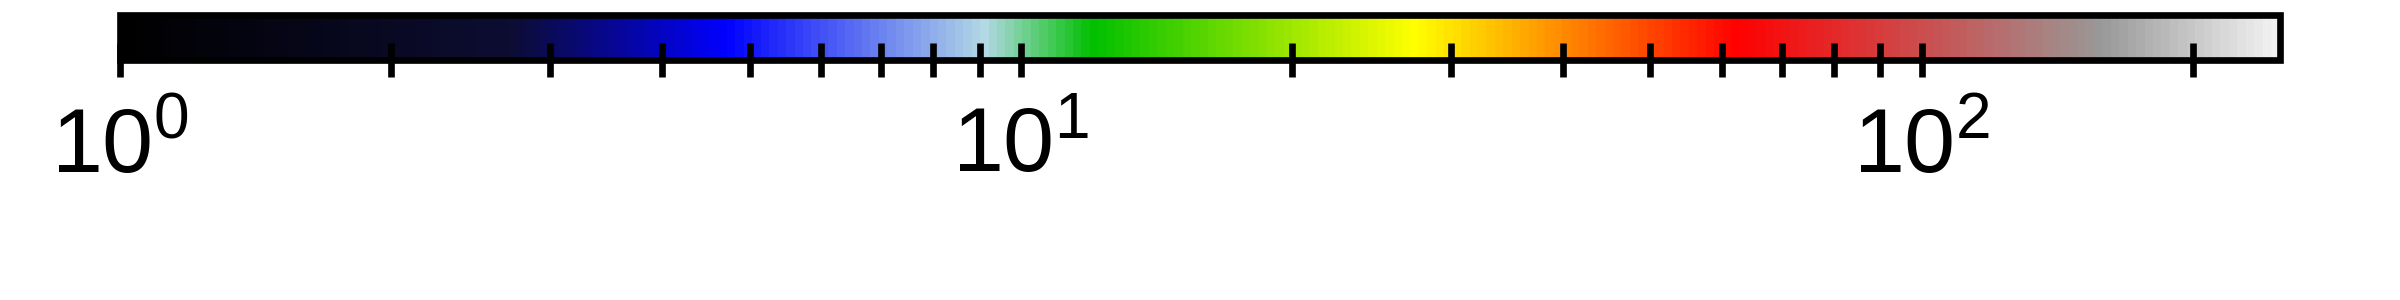
\includegraphics{monolayers_ML-Ac-CoFe-C_GISANS_SVcbar_negField}
    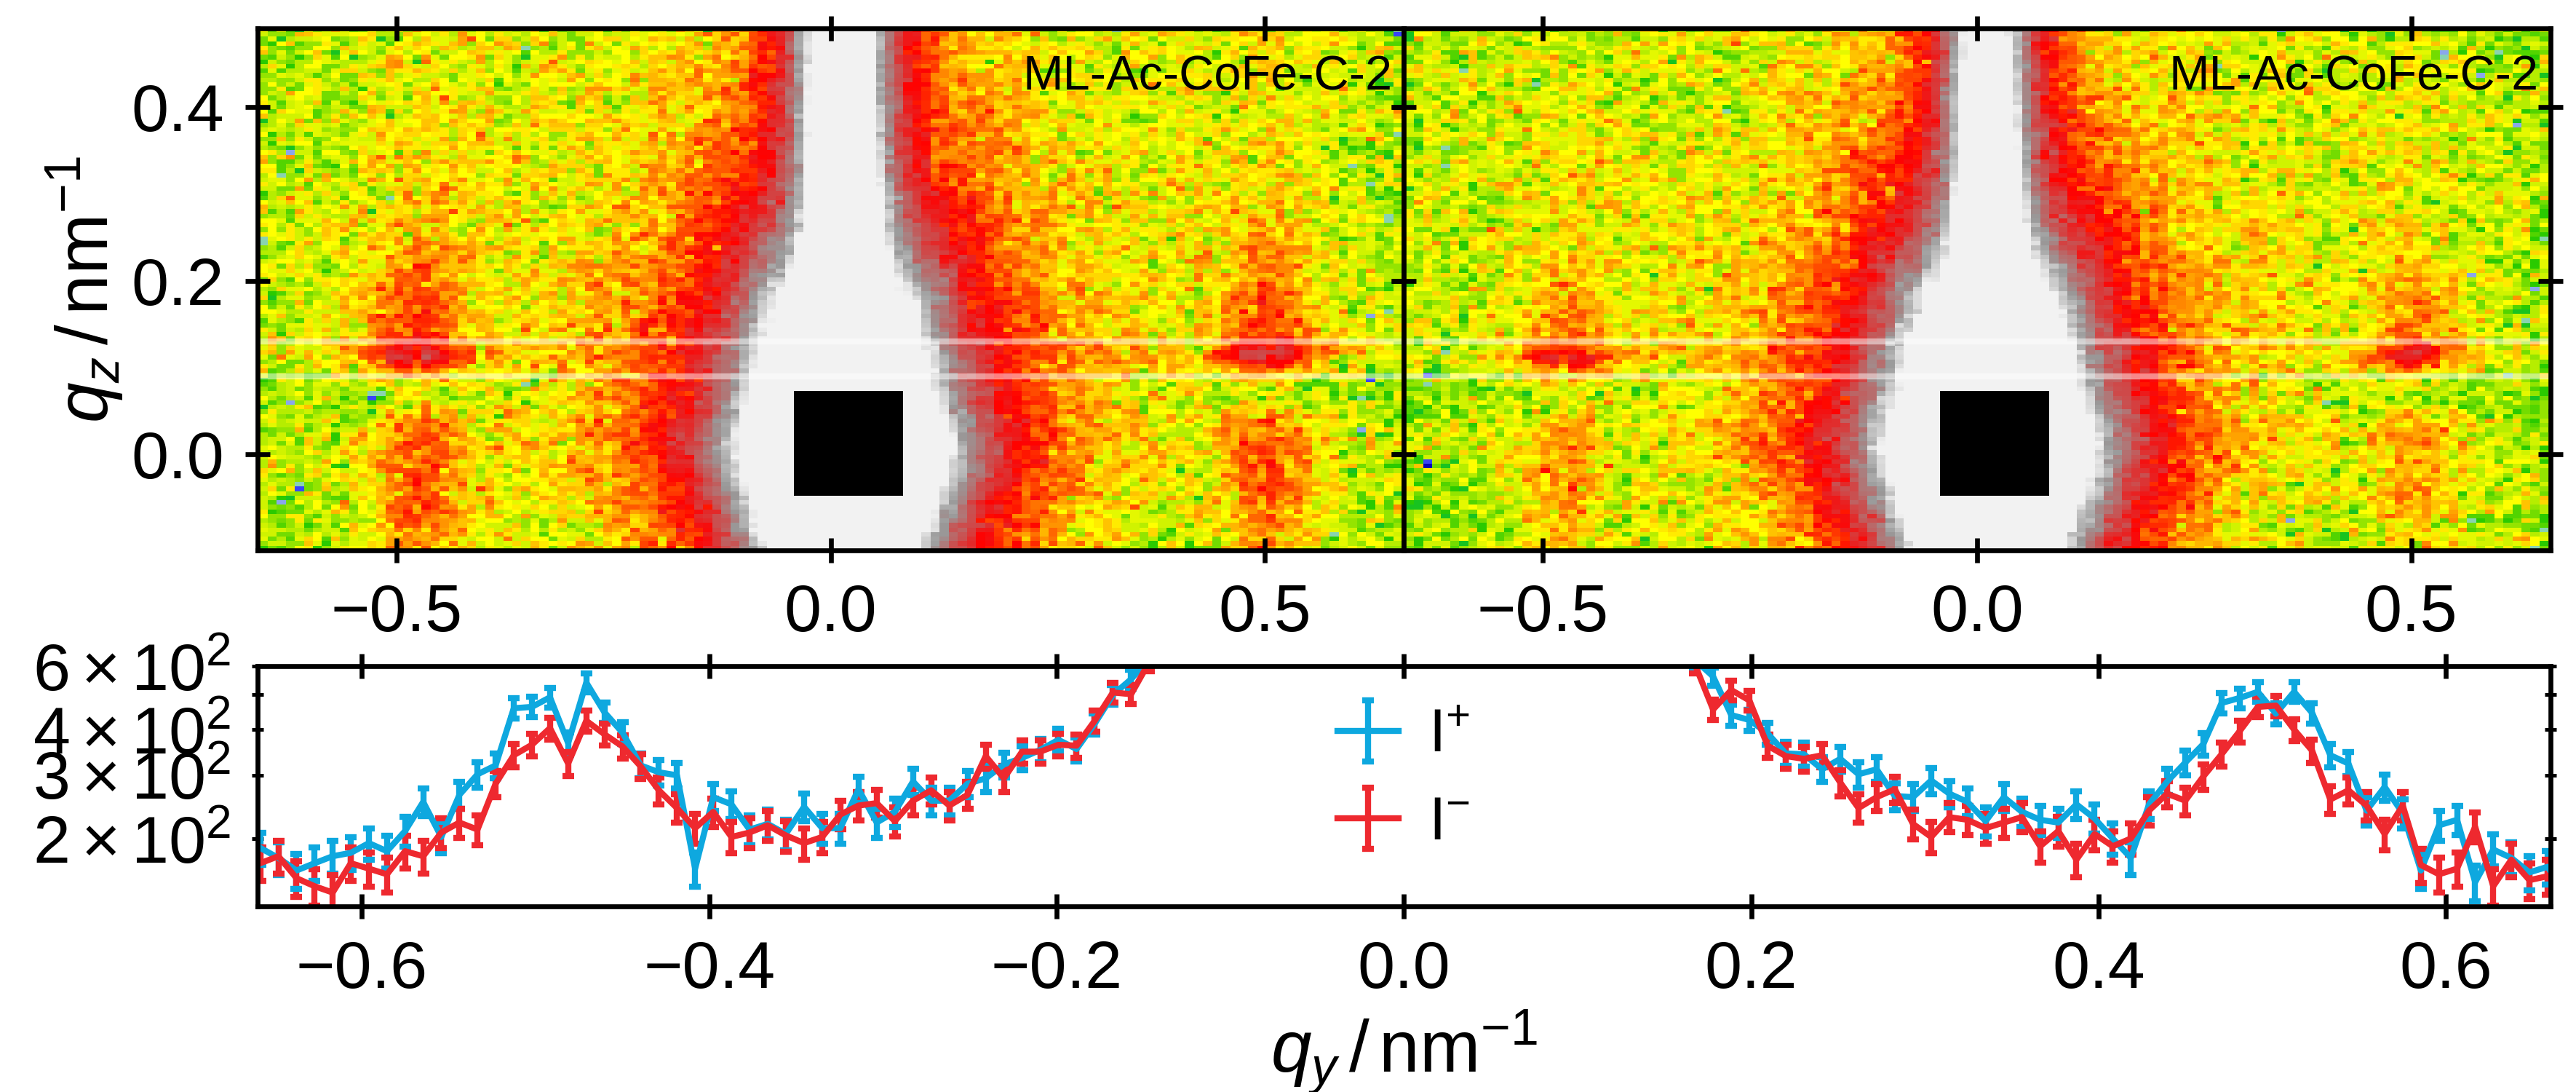
\includegraphics{monolayers_GISANS_ML-Ac-CoFe-C-2_ZFC5K_negField}
    \caption{\label{fig:monolayer:magneticStructure:negativeField}PolGISANS of ML-Ac-CoFe-C-2 after ZFC and saturation in a magnetic field of $4 \unit{T}$ analogue to \reffig{fig:monolayer:magneticStructure:polGisans5KZFC} measured in a negative magnetic field $-200 \unit{mT}$ applied parallel to the neutron beam. The left detector image shows $I^{+}$ and the right image $I^{-}$. The lower plot shows the Yoneda band of both detector images.}
  \end{figure}

  Going further along the hysteresis by applying a negative field of $-200 \unit{mT}$ parallel to the neutron beam the data shown in \reffig{fig:monolayer:magneticStructure:negativeField} is obtained.
  Here, a magnetic contrast between $I^{+}$ and $I^{-}$ is visible in both the detector images and the Yoneda band.
  It is visible that $I^{+} > I^{-}$ in the peak, where $I^{+}$ is the measurement performed with the radio flipper turned off and $I^{-}$ with the radio flipper on.
  Generally, the polarization direction $\vec{P}$ of the beam is defined as parallel to the applied field $\vec{H}$.
  This means, as the magnetic field is negative the sign of the magnetization has to be switched in the simulation, and thereby the measured case corresponds to the ferromagnetic state described in the first simulation of \reffig{fig:monolayers:gisans:simulationAlternating}.
  This is the state which would have primarly been expected in the remanent state before but was not observed.
  Possibly the discrepancy can be explained by a sub-optimal beam polarization during the measurement.
  With the negative magnetic field measurement, it can be concluded however that the magnetization of the sample is preferentially parallel to the neutron beam direction at low fields.

  \begin{figure}[tb]
    \centering
    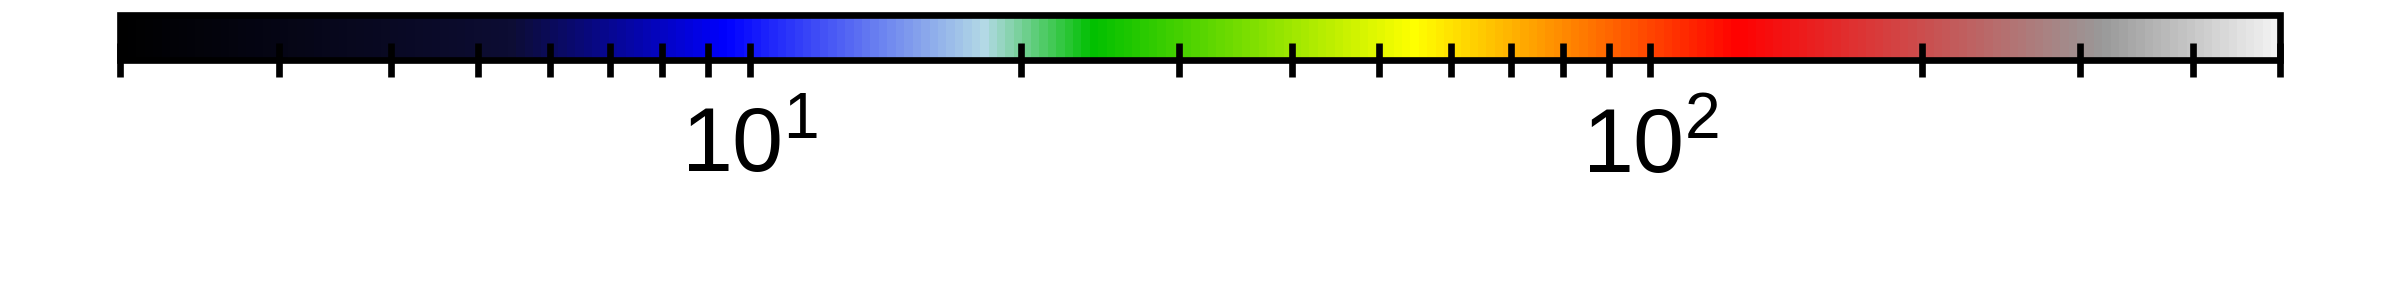
\includegraphics{monolayers_ML-Ac-CoFe-C_GISANS_SVcbar_perpendicularBeam}
    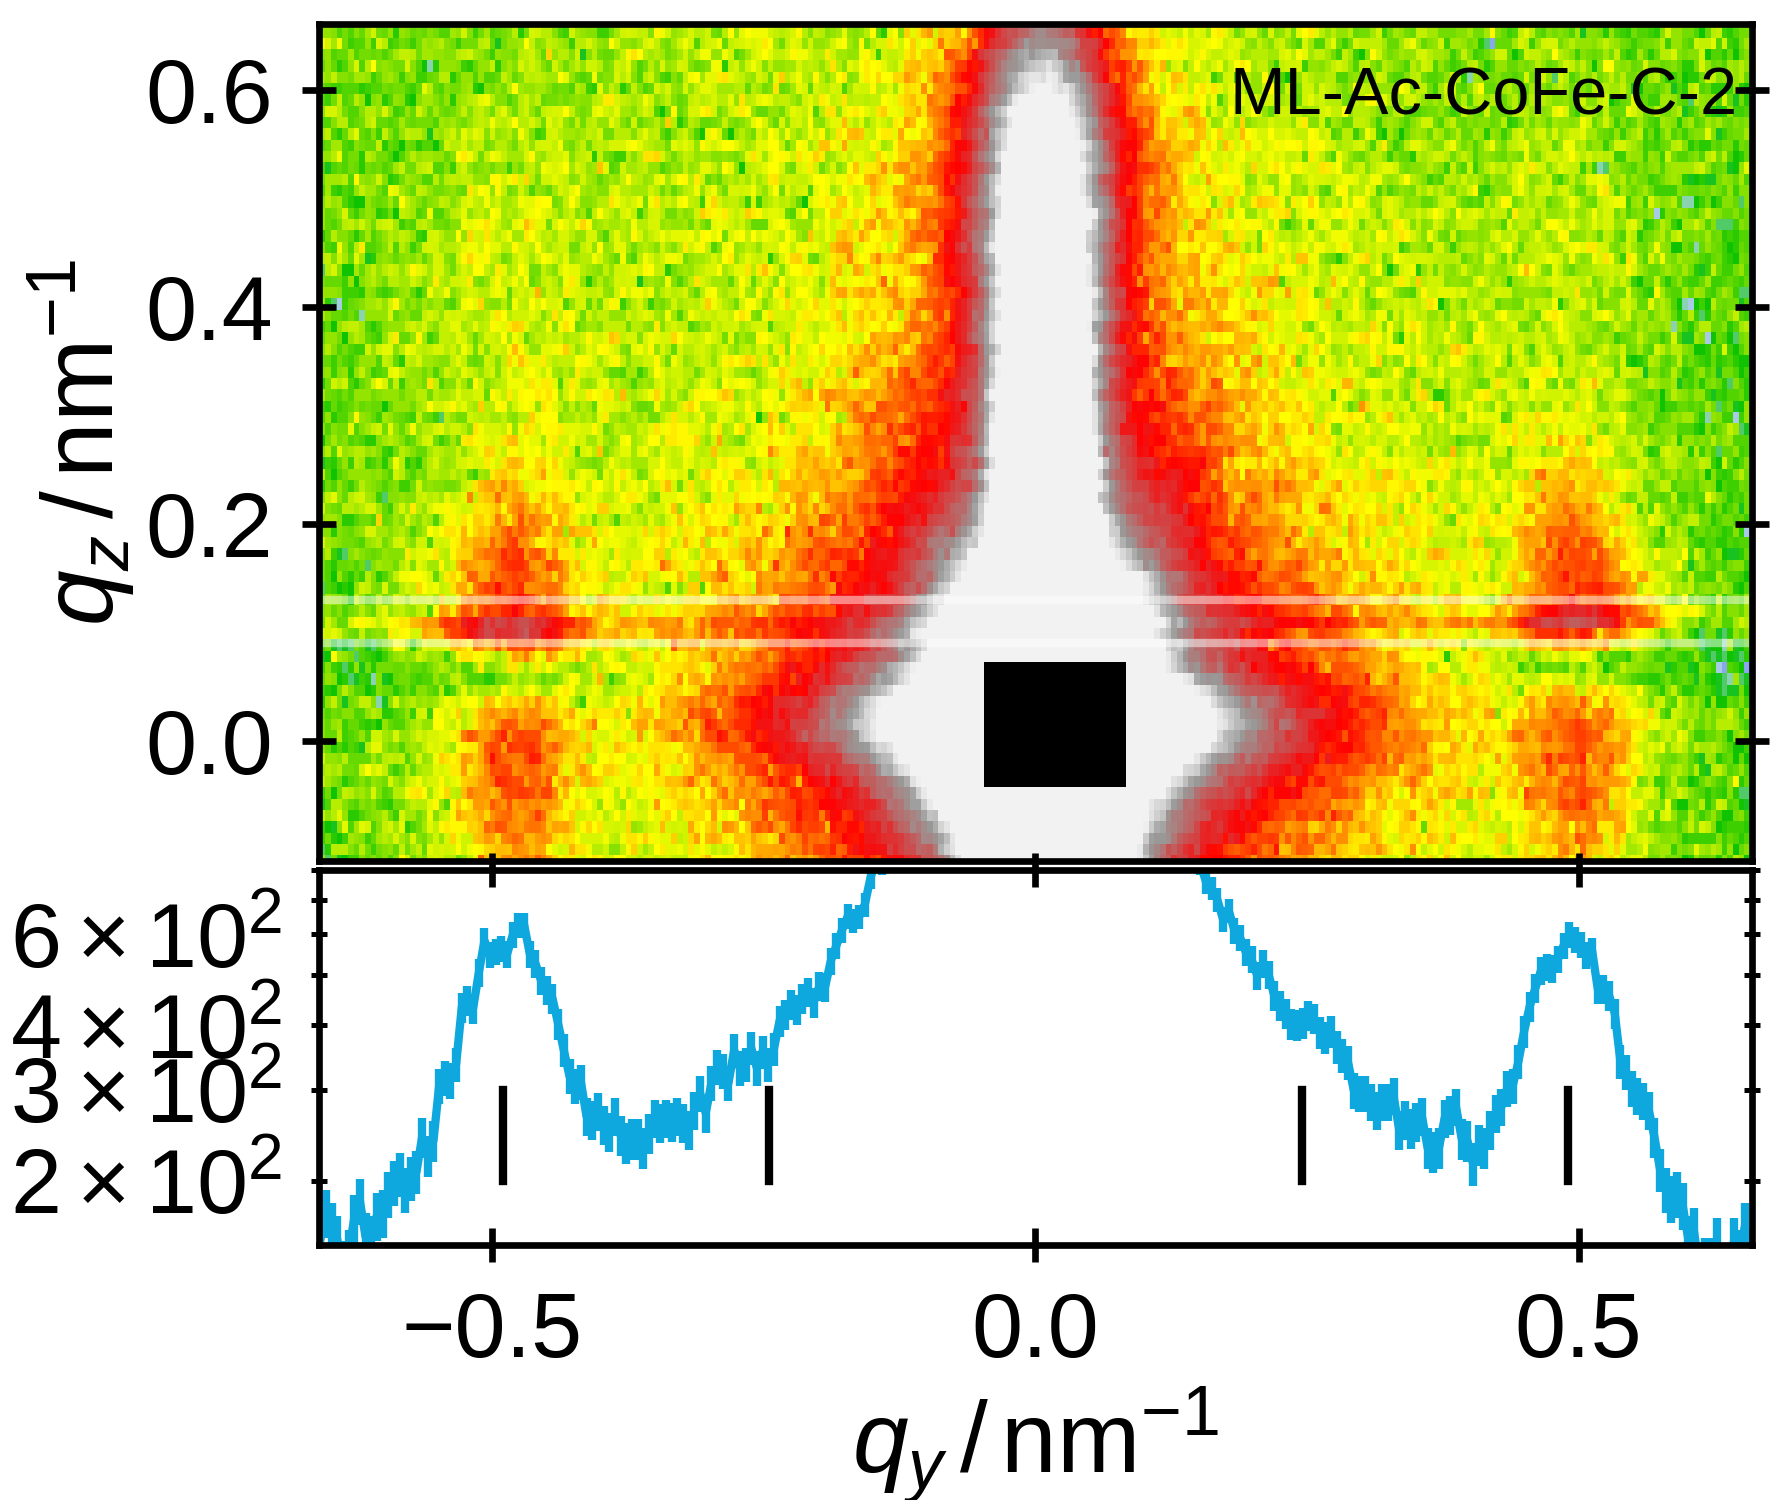
\includegraphics{monolayers_GISANS_ML-Ac-CoFe-C-2_ZFC5K_Unpolarized_GF}
    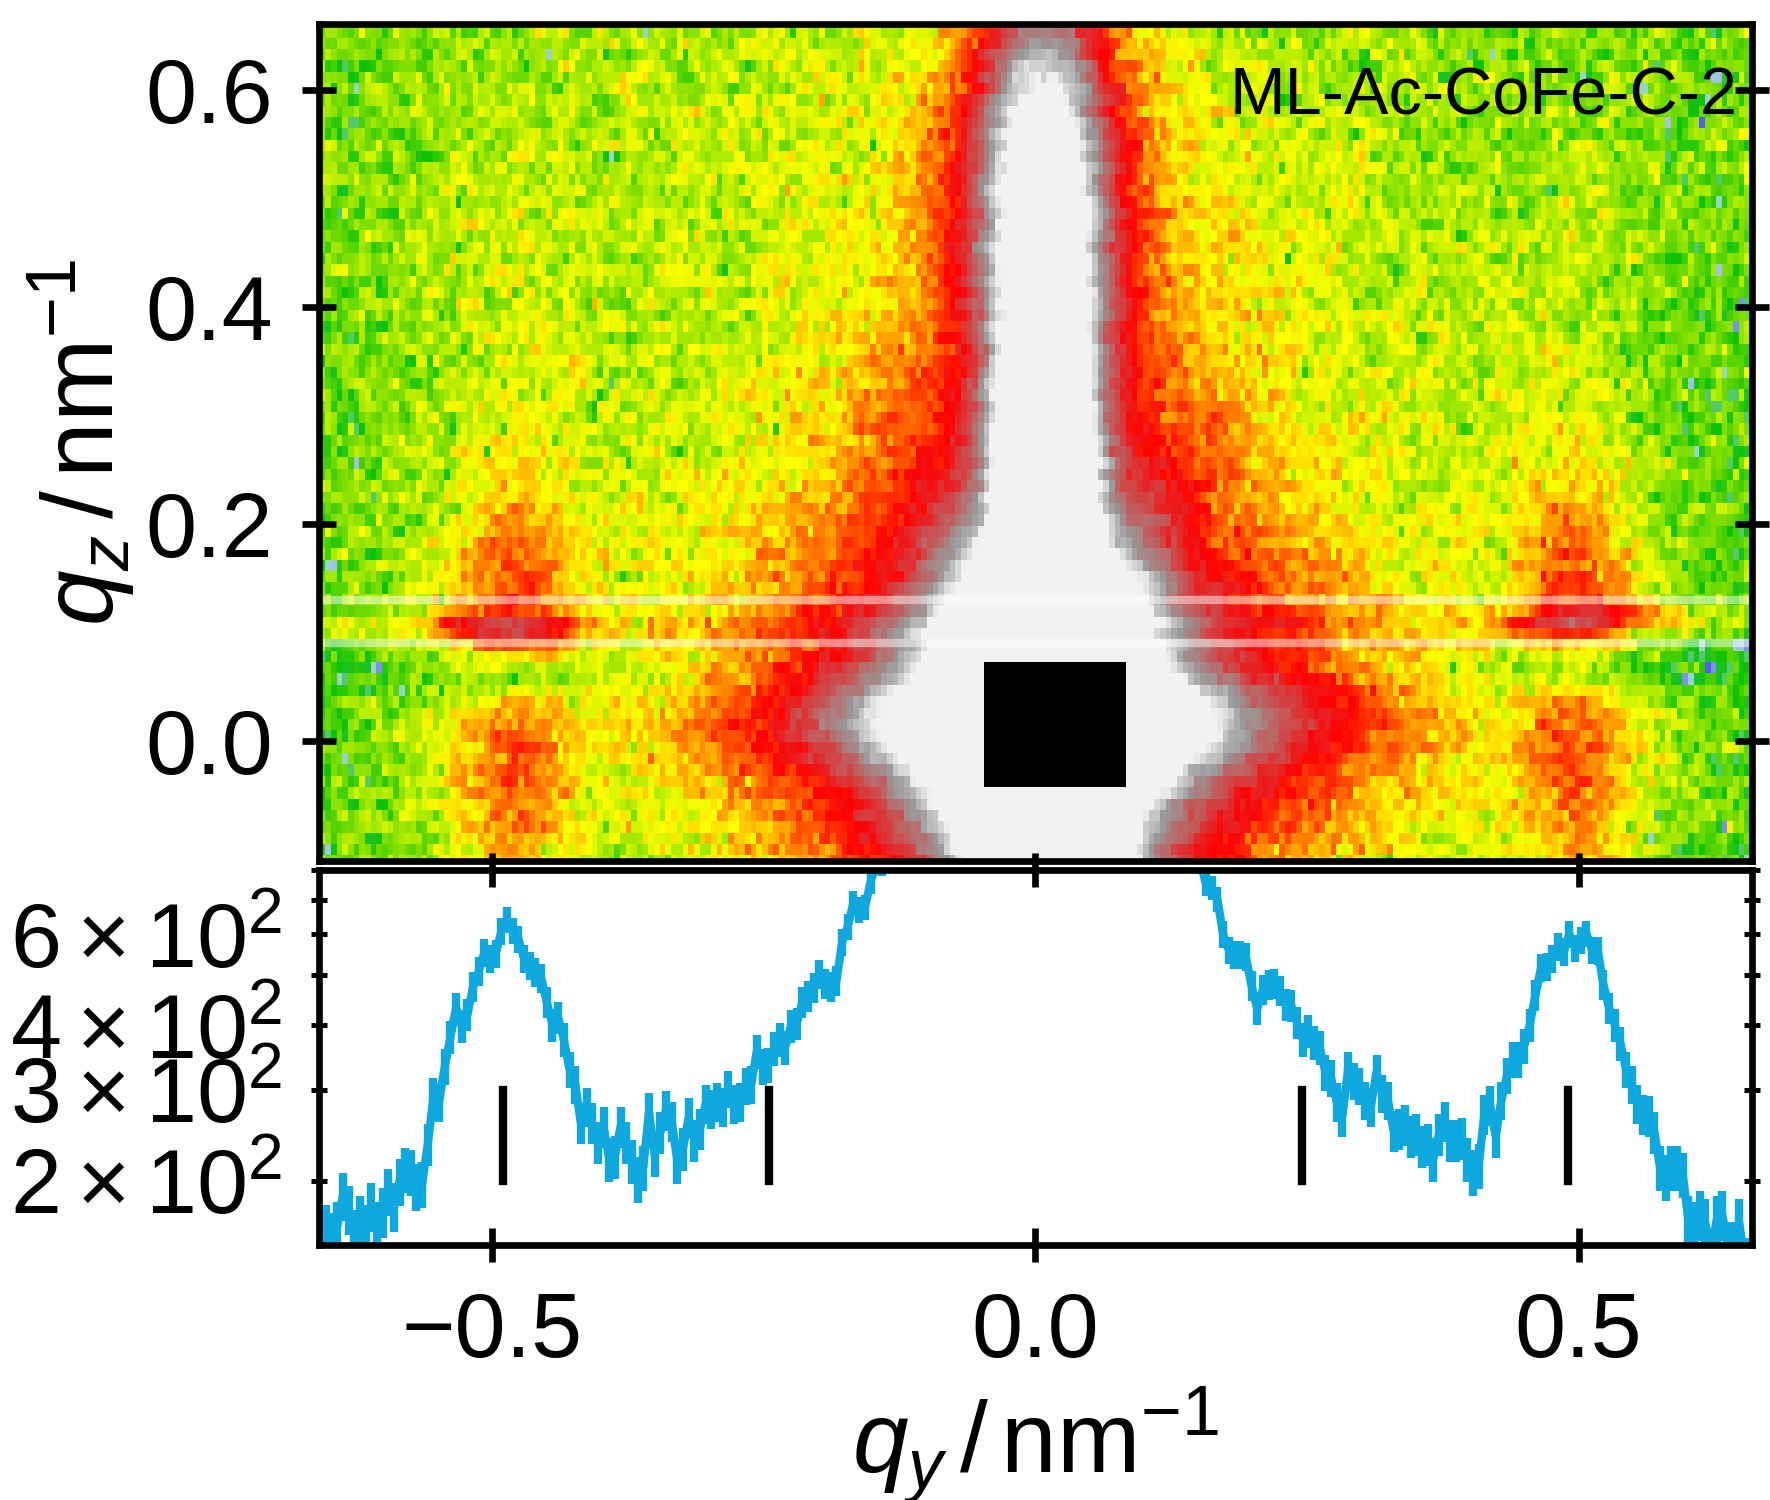
\includegraphics{monolayers_GISANS_ML-Ac-CoFe-C-2_ZFC5K_Unpolarized_Remanence}
    \caption{\label{fig:monolayer:magneticStructure:Gisans5KZFCperpendicular}GISANS of ML-Ac-CoFe-C-2 after zero-field cooling to $5 \unit{K}$. The sample is measured initially at the guide field of $5 \unit{mT}$ (left) and in remanence after application of a $4 \unit{T}$ field in the sample plane, perpendicular to the neutron beam. The lower plots show the projection of the Yoneda band.}
  \end{figure}

  To study whether a significant number of spins flips by $90 ^\circ$ after removal of the magnetic field to form antiferromagnetically coupled lines in the square lattice, \reffig{fig:monolayer:magneticStructure:Gisans5KZFCperpendicular} shows the same measurement as discussed before but with the $4 \unit{T}$ field applied perpendicular to the beam in the sample plane.
  In this configuration, no magnetic splitting from a super ferromagnetic phase in the sample would be expected.
  Therefore the measurement is performed without distinction of the incoming neutron polarization to improve the counting statistics and to focus on whether antiferromagnetic peaks emerge.
  With good will, a slight increase in intensity is visible in the measurements around the expected region for the super antiferromagnetic peak at $q_y \eq 0.25 \unit{nm^{-1}}$.
  The peak can, however, also be considered as a statistical fluctuation as it is not symmetrically visible in the negative $q_y$ range.
  If it is considered to be a signature of SAFM coupling, the strong smearing and low intensity suggest that the domain of super antiferromagnetically coupled regions on the sample have a small extension and might therefore be difficult to observe.
  \\

  Concludingly the measurements have shown multiple results.
  For one, the measurements confirm that the material of a drop-casted monolayer in a polGISANS experiment is already enough to provide a clearly measurable signal in a reasonable amount of measuring time.
  For the other, the magnetic splitting in the measurement with the magnetic field applied antiparallel to the beam direction confirms that a major part of the magnetic moment remains aligned with the originally saturating field direction.
  Unclear remains however, whether a true super antiferromagnetic signal is observed as the obtained data is not providing a concluding signal.
  It appears that it may be necessary to prepare higher quality monolayers and possibly measure with even longer counting times to make a concluding observation.

  % Additional measurements performed at $250 \unit{K}$ with the applied field parallel and perpendicular to the beam in the sample plane show no different results (not shown) and thus it can be concluded that if any super antiferromagnetic peak is present in the sample, it is heavily smeared out and hidden in the background.


\end{document}